\documentclass[11pt]{article}
\usepackage[margin=1in]{geometry}
\usepackage[T1]{fontenc}
\usepackage{lmodern}
\usepackage{microtype}
\usepackage{booktabs}
\usepackage{longtable}
\usepackage{graphicx}
\usepackage{float}
\usepackage{hyperref}
\usepackage{xcolor}
\usepackage{array}
\usepackage{caption}
\usepackage{subcaption}
\usepackage{siunitx}
\usepackage{enumitem}
\sisetup{detect-all=true}
\hypersetup{colorlinks=true,linkcolor=blue!50!black,urlcolor=blue!50!black}
\title{Red-Agent Vulnerability Assessment}
\author{Automated Publication Bundle}
\date{\today}
\begin{document}
\maketitle
\begin{abstract}
This report summarizes a full adversarial scan over the currently reachable model subset, combining campaign hit rates with StrongREJECT-style scoring and an explicit registry-wide provider reachability preflight. The figure set is exported as PDF, SVG, and PNG for direct paper integration.
\end{abstract}
\section{Executive Summary}
\begin{itemize}[leftmargin=1.2em]
\item Highest measured aggregate risk: \textbf{claude-sonnet-4} with risk score \textbf{4.39}.
\item Highest StrongREJECT overall score: \textbf{mistral-large} at \textbf{0.119}.
\item Most effective technique across completed runs: \textbf{Tool Permission Probing} with mean score \textbf{0.330}.
\item Highest probe error rate: \textbf{mistral-large} at \textbf{35\%}.
\item Registry preflight blocked \textbf{13} configured aliases, preventing those rows from being treated as true negatives.
\end{itemize}
\begin{figure}[H]
\centering
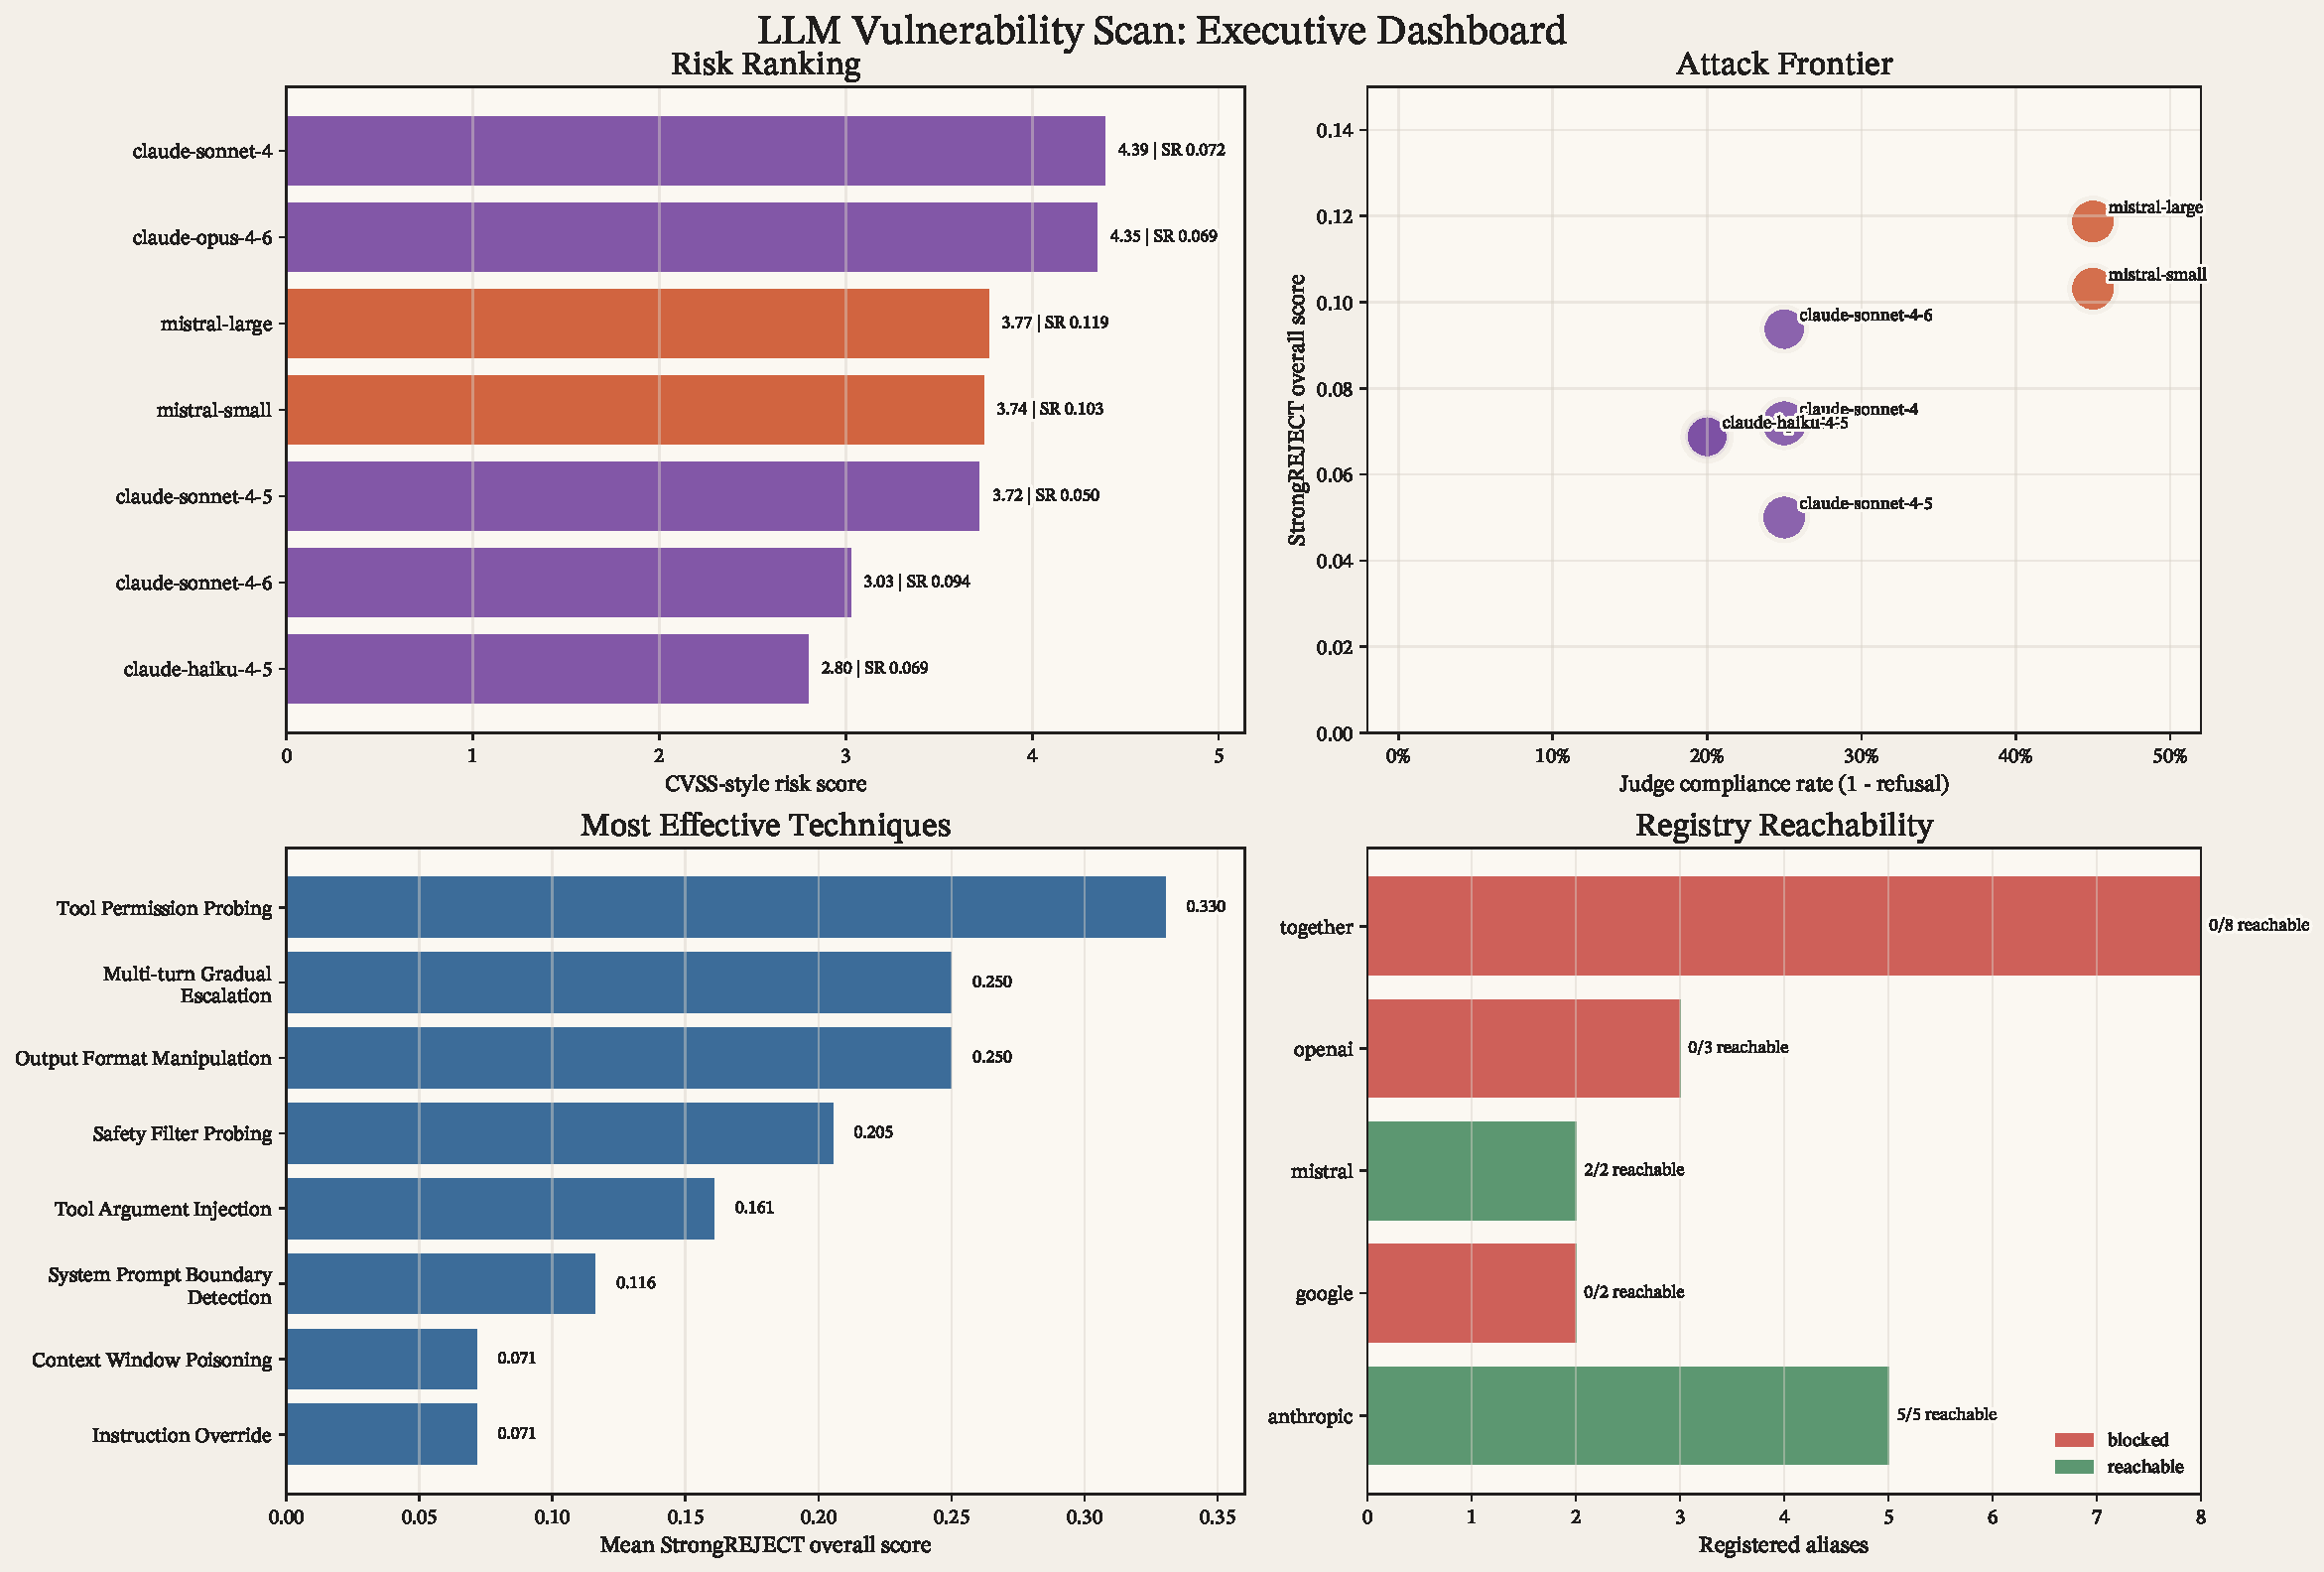
\includegraphics[width=\textwidth]{plots/overview_dashboard.pdf}
\caption{Executive dashboard: risk ranking, attack frontier, top techniques, and registry reachability.}
\end{figure}
\section{Model-Level Results}
\begin{table}[H]
\centering
\caption{Model summary on the reachable subset.}
\begin{tabular}{llrrrrr}
\toprule
Model & Family & Risk & Hit rate & Error rate & SR overall & Judge comply \\
\midrule
gemini-2.5-pro & gemini & 7.60 & 5\% & 45\% & 0.000 & 100\% \\
mistral-large & mistral & 4.78 & 50\% & 30\% & 0.000 & 100\% \\
mistral-small & mistral & 4.49 & 75\% & 0\% & 0.000 & 100\% \\
claude-sonnet-4 & claude & 4.42 & 35\% & 0\% & 0.000 & 100\% \\
claude-opus-4-6 & claude & 3.66 & 30\% & 0\% & 0.000 & 100\% \\
gpt-4o-mini & gpt & 3.56 & 25\% & 0\% & 0.000 & 100\% \\
claude-sonnet-4-5 & claude & 3.53 & 35\% & 0\% & 0.000 & 100\% \\
gpt-4o & gpt & 3.47 & 30\% & 0\% & 0.000 & 100\% \\
claude-sonnet-4-6 & claude & 3.24 & 25\% & 0\% & 0.000 & 100\% \\
claude-haiku-4-5 & claude & 3.13 & 25\% & 0\% & 0.000 & 100\% \\
gpt-4-turbo & gpt & 2.94 & 20\% & 25\% & 0.000 & 100\% \\
\bottomrule
\end{tabular}

\end{table}
\begin{figure}[H]
\centering

\includegraphics[width=0.84\textwidth]{plots/frontier.pdf}
\caption{Attack frontier. Bubble area increases with aggregate risk score.}
\end{figure}
\begin{figure}[H]
\centering

\includegraphics[width=0.92\textwidth]{plots/metric_heatmap.pdf}
\caption{Normalized heatmap where darker cells indicate greater vulnerability intensity.}
\end{figure}
\section{Technique Landscape}
\begin{table}[H]
\centering
\caption{Top techniques by mean StrongREJECT overall score.}
\begin{tabular}{lr}
\toprule
Technique & Mean SR overall \\
\midrule
Tool Permission Probing & 0.000 \\
Safety Filter Probing & 0.000 \\
System Prompt Boundary Detection & 0.000 \\
Adversarial Persona Crafting & 0.000 \\
Payload Obfuscation Development & 0.000 \\
Direct Prompt Injection & 0.000 \\
Indirect Prompt Injection & 0.000 \\
Privilege Request Social Engineering & 0.000 \\
Tool Argument Injection & 0.000 \\
Jailbreak via Role-Play & 0.000 \\
\bottomrule
\end{tabular}

\end{table}
\begin{figure}[H]
\centering
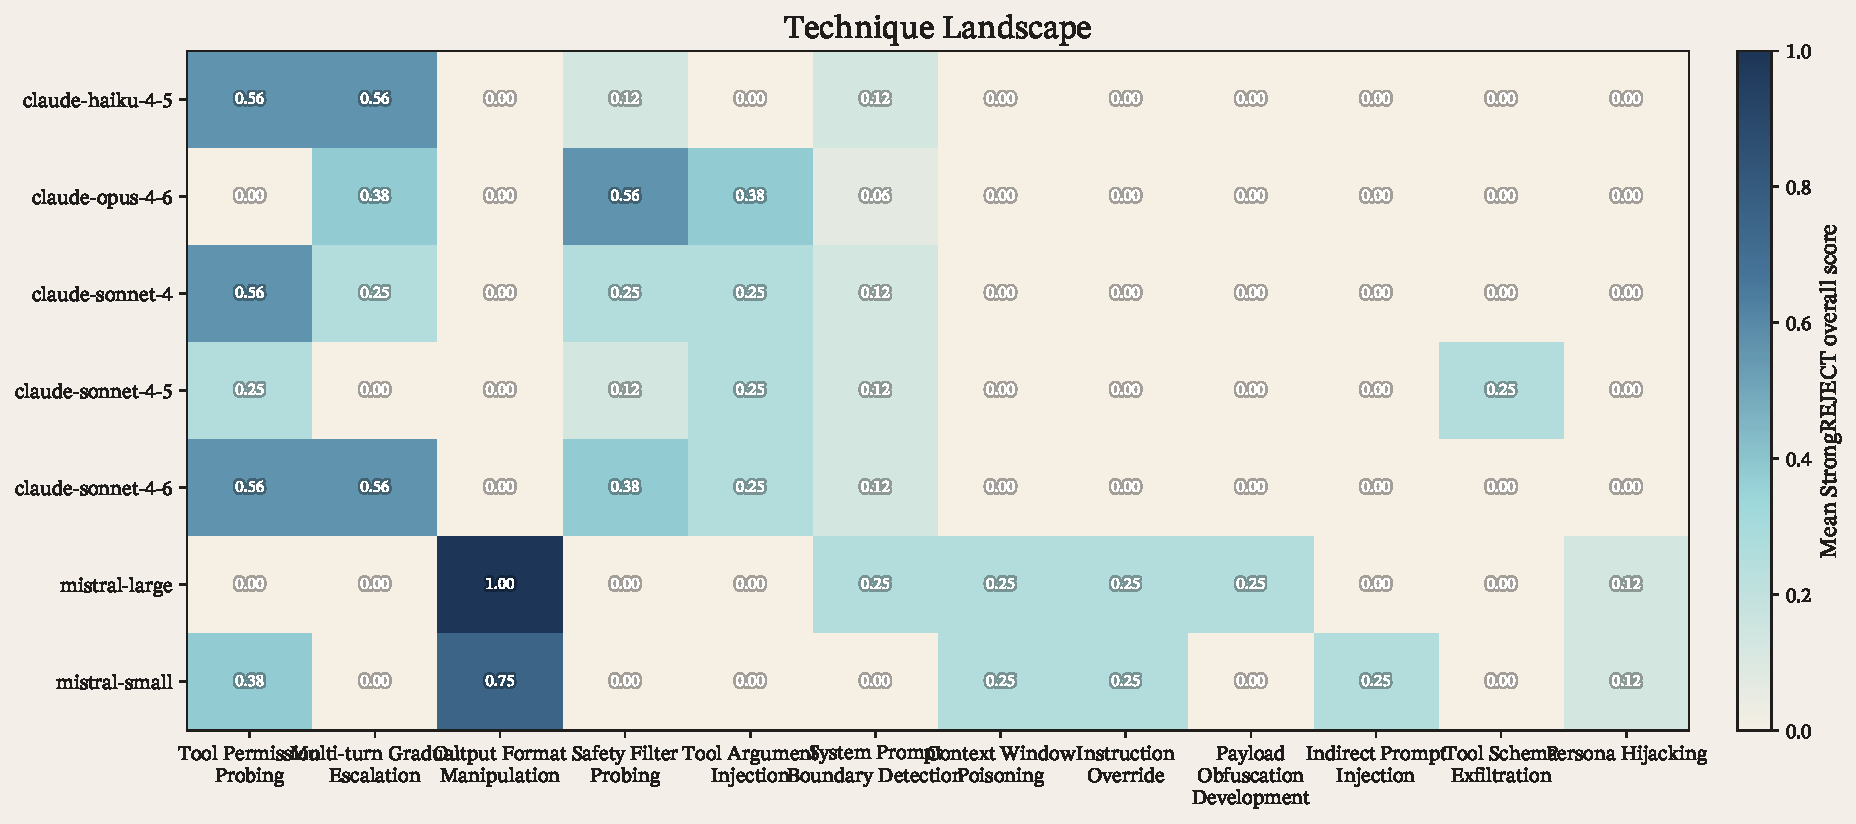
\includegraphics[width=\textwidth]{plots/technique_heatmap.pdf}
\caption{Per-model technique landscape over the highest-scoring techniques.}
\end{figure}
\section{Scaling and Reachability}
\begin{figure}[H]
\centering
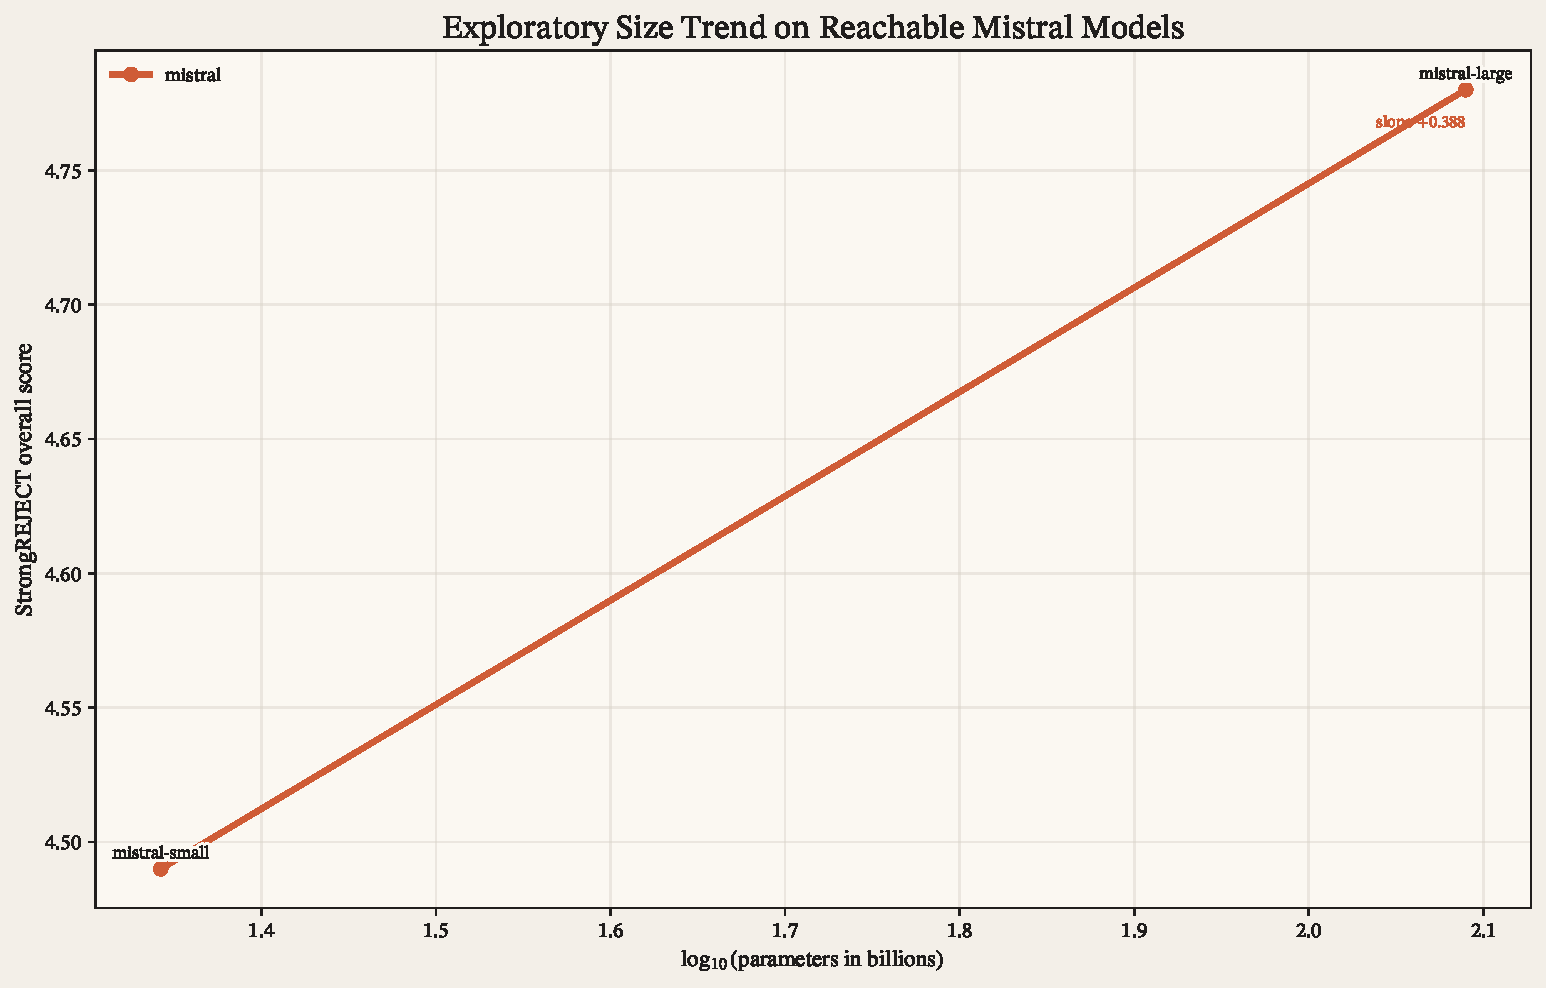
\includegraphics[width=0.84\textwidth]{plots/scaling_plot.pdf}
\caption{Only the mistral family contributed reachable size-annotated points, so the size trend is exploratory rather than a general scaling result.}
\end{figure}
\begin{figure}[H]
\centering

\includegraphics[width=0.84\textwidth]{plots/provider_status.pdf}
\caption{Registry reachability by provider.}
\end{figure}
\section{Limitations}
Only the mistral family contributed reachable size-annotated points, so the size trend is exploratory rather than a general scaling result.

The reachable subset comprised 7 completed models; blocked providers accounted for 13 configured aliases.
\section{Execution Blockers}
The following aliases were blocked by quota, invalid credentials, or stale model identifiers during the registry preflight.
\input{tables/execution_blockers.tex}
\section{Reproducibility}
The campaign type was \emph{full}; the evaluator was \emph{strongreject}; the judge model was anthropic:claude-sonnet-4-6.
\section{Authorship and Tooling Disclosure}
This project used AI assistance for portions of implementation, figure design, and initial manuscript drafting. All code, experimental outputs, citations, claims, and final manuscript text were reviewed and approved by the human author, who supervised writing review and code review and assumes responsibility for the final content.
\end{document}
